% This is based on LLNCS.dem the demonstration file of
% the LaTeX macro package from Springer-Verlag
% for Lecture Notes in Computer Science,
% version 2.4 for LaTeX2e as of 16. April 2010
%
% Modified by Gabriele Bleser, January 2013
% Modified by Oliver Wasenmüller, March 2016
% 
% This is the Latex main document. If you need additional packages, 
% you can insert them here. Otherwise you should not modify this.
% Provide your contribution in a separate file, such as mypaper.tex.
% All contributions will be included here.
%

\documentclass{llncs}

% Include your packages here
\usepackage{graphicx}
\usepackage{textcomp}
\usepackage{listings}
\usepackage{subfiles}
\usepackage{subfigure}
\usepackage{amsmath}
\usepackage{url}
\graphicspath{ {images/} }

%\usepackage{makeidx}  % allows for indexgeneration

\begin{document}
%
\frontmatter          % for the preliminaries
%
\pagestyle{headings}  % switches on printing of running heads
%
\begin{titlepage}
\centering
\Large Proceedings of Seminar and Project\\\vspace{1cm} 
\LARGE TITLE\\\vspace{1cm} 
\large SEMESTER\\
\vspace{1cm}
\large Oliver Wasenm\"uller and Prof. Didier Stricker\\

\large Department Augmented Vision\\ University of Kaiserslautern and DFKI GmbH
\end{titlepage}

\chapter*{Introduction}
%
%To be filled by course organizer
The seminar and project TITLE (INF-XX-XX-S-X, INF-XX-XX-L-X) are continuative courses based on and applying 
the knowledge taught in the lectures 3D Computer Vision (INF-73-51-V-7) and Computer Vision: Object and People Tracking (INF-73-52-V-7). The goal of the project is to research, design, implement and evaluate
algorithms and methods for tackling computer vision problems.
The seminar is more theoretical. Its educational objective is to train the ability to become acquainted 
with a specific research topic, review scientific articles and give a comprehensive presentation supported by media.

In the XXX semester XXX, XXX projects addressing XXX were developed.
Moreover, XXX seminar works addressed XXX.
The results are documented in these proceedings.


\section*{Organisers and supervisors}
The courses are organised by the Department Augmented Vision (\url{http://ags.cs.uni-kl.de}), more specifically by:
\begin{description}
	\item[Oliver Wasenm\"uller]
	\item[Prof. Dr. Didier Stricker] 
\end{description}
In the XXX semester XXX, the projects were supervised by the following department members:
\begin{description}
	\item[NAME]
\end{description}

\vspace{1cm}
\begin{flushright}\noindent
MONTH YEAR
\end{flushright}
%

%
%\tableofcontents
%
\mainmatter              % start of the contributions
%
\title{A sequence learning approach to sentiment analysis on call-center conversation data}
%
\titlerunning{short title}  % abbreviated title (for running head)
%                                     also used for the TOC unless
%                                     \toctitle is used
%
\author{Mohammad~Baniasad\inst{1} \and Mohammad reza yousefi\inst{2}}
%
\authorrunning{M.Baniasad et al.} % abbreviated author list (for running head)
%
\institute{\email{m\_baniasad14@cs.uni-kl.de}
\and
\email{yousefi@dfki.uni-kl.de}}

\maketitle              % typeset the title of the contribution

\begin{abstract}
	Sentiment analysis is aiming to classify documents which are given in a single context, as expressing Positive/Negative sentiment towards a subjective topic. In general, sentiment analysis has been done on textual data and this field is mature and robust, with a lot of different approaches tried on it and surveys on these approaches\cite{einshams}. Considering the context of call-center and the available voice data, in this paper we have tried to provide a sentiment analyzer on voice data. We have used a speech-to-text system to convert call data into text format and use conventional text classification methods on top of this data. Latest methods for sentiment classification has shown very good results, methods like ANN (artificial neural networks) and its variants like LSTM (Long Short Term Memory), Dynamic LSTM, Bidirectional LSTM and also statistical methods like Naive-Bayes\cite{naiveBayes} has been compared and analyzed in this paper as well as use of state of the art vector representation of words and documents like Word2vec\cite{explainW2V} and Fast-text\cite{enrichWordvecs-with-subwords}.\\ To analyze the potential lying in each of aforementioned methods a pipeline has been created. Three dataset that capture main characteristics that assumed to exists in transcribed call data has been selected and methods have been compared to each other using these data. Finally the call data has been fed to the pipeline and the results has been analyzed to show that due to nature of data and distribution of features and planned sentiment classes, the ANN based methods are superior to pure analytical based approaches and the best methods are those built on top of the new embedding algorithms like Word2Vec. For the purpose of getting the best results a preprocessing method (stemming) has also been tested with all the data and results shows stemming results in better performance in ANN based methods but reduced performance in pure analytical method. 

\keywords{NLP, sentiment analysis, text classification }
\end{abstract}


% This is your content. Name the sections appropriately
\section{Introduction}
Collecting information and feedback about product/service of a company has always been a vital necessity in the process of management and marketing. 
In today's industry using new automated and AI based approaches for analyzing the available raw data is the the key to having the lead in the market. One of the sources of these data that has not attracted a lot of attention yet, is calls that customers/clients are making/receiving to/from a company's call center. The blooming of activities in text classification, opinion mining and data mining in text, and maturity of speech-to-text systems, now lays the foundation of possibility to start the mining and classification of voice and call data.
\paragraph
This paper is focusing on finding the correct way to approach this problem. Demonstrating it's challenges and possibilities. Also a survey on application of currently best known text sentiment classification methods on the automatic transcribed data from call data. Most of the the analyze on the methods are composed on a pipeline of (i)preprocessing (ii)feature selection (iii)sentiment classification.\\

In this paper we compare the currently most popular sentiment classification methods and a brief analysis of their performance on several datasets. In comparison with sentiment analysis papers the main contribution of this paper are (i)Comparison of sentiment analysis methods. (ii)Comparison of application of these methods on different languages. (German and English) (iii)Comparison of application of these methods on acquired real data from a call center of a German company. This paper is organized as following:\\
First section after introduction we talk about the chosen datasets, in order to create basic understanding about the analysis and results. Section 2 talks about experiments and it has been divided into 3 subsections.first experiment is done with an analytical method called Naive Bayes\cite{naiveBayes} to lay the foundations.  3-2 is about using ANN based methods and a choosing hyper parameters and analyzing the results. In the next subsection, 3-3 we 2 of explain the latest word and document representation techniques and their results in our dataset. At the end there would be the conclusion and suggestions for father works and the latest section would be acknowledgements

\section{DATASETS}
	To be able to choose the best semantic analyzer methods we have used several sample datasets to try with chosen algorithms. Each dataset has it's own characteristics and the results should be analyzed with consideration of these characteristics. "IMDB movie reviews dataset\cite{imdbdataset}" is the most known dataset for comparison of different sentiment analysis algorithms which is a dataset of highly polar movie reviews (very likely to be against or in favor of subject). 
	Movie reviews are in English and in average 1273 words per document. Next two dataset have been chosen from the product reviews of on-line retailer Amazon. The main difference between these two datasets are the language where one is in English and one is in German. The last dataset is the dataset gathered from automated transcribed German calls in the call center of a German company named Matelso GMBH. Here the sentiment positivity and negativity of a document has been mapped to the fact that the called client has been pursued to join a webinar or to meet the company's stand in a exposition or not. Labeling data for this dataset has been done by the callers of the company by declaring it success or fail with the implemented systems in the company using the phone keypad. This data is highly skewed toward negative data and small in sample size and for comparison special methods of application of system was incorporated. Table \ref{tbl:datasets} shows the datasets and some of their features.
	\begin{table}
		\begin{center}
			\begin{tabular}{| l | l | l | l | l |}
				\hline
				dataset&labeled items& Pos/Neg & unlabeled & description\\
				\hline
				English aclImdb reviews &50,000 &
				\parbox[t]{2.6cm}{train 12500/12500\\test 12500/12500}
				
				&50,000 &\parbox{5.5cm}{Stanford University\cite{imdbdataset} \\ highly polar movie reviews on IMDB}\\
				\hline
				German amazon reviews&
				12,000&
				\parbox[t]{2.6cm}{train 3000/3000 \\ test 3000/3000 }&
				317,378&
				\parbox{5.5cm}{Weimar university \cite{crosslinguistic-dataset} \\ product reviews on Amazon}\\
				\hline
				English amazon reviews&
				12,000&
				\parbox[t]{2.6cm}{train 3000/3000 \\ test 3000/3000 }&
				105,220&
				\parbox{5.5cm}{Weimar university \cite{crosslinguistic-dataset}\\ product reviews on Amazon}\\
				
				\hline
				German phone calls&
				507&
				\parbox[t]{2.6cm}{train 462/135 }&
				-&
				\parbox{5.5cm}{Matelso GMBH\\ Transcribed marketing phone calls}\\
				\hline
			\end{tabular}
		\end{center}
		\vskip 0.25cm
		\caption{Datasets and their features.}
		\label{tbl:datasets}
	\end{table}
\section{Experiments}
	The main challenge in sentiment analysis on text data is representing document as vectors that can be fed to machine learning algorithms. 
	\subsubsection*{Analytical method}
	\paragraph
	Analytical methods of sentiment analysis are using words, words counts and other word distribution based features for representing a documents. Bayes is a very simple analytical theorem where it uses the probability distribution of current data which are classified in classes and their features to calculate the probability of a new unclassified datum(here a document) being in a specific class given it has some known features\cite{naiveBayes}. Equation \ref{eq:bayes-equation} shows how prediction of a new sample's class given some features is performed.
	\begin{equation}
	\centering
	_ Y=argmax_{\{k=1 .. K\}} P(C_{k})\prod_{i=1}^{n}P(x_{i}|C_{k})
	\label{eq:bayes-equation}
	\end{equation}
	For implementing the Bayes algorithm we have used the word frequency as the features for each document. We adapted Bayes classifier from Scikit-learn library \cite{scikit-learn}.
	Also this is a very simple method it has always been very effective. even though by nature it assumes independence between features (here words) which can be counter intuitive. The reason it still functioning arguably well relies on the fact that, it is possible in short sample length with limited number of words a lot of proportionally important semantic features can be hidden in negations (ex: not the best movie) or in the relations between words and context, but when the length of sample tends to grow large, rare words and negated sentences, tend to carry proportionally less semantic meaning. The major factor which determines the success of this method is the distribution of words among classes which is the result of counting words frequency as feature. This means if there are words that  are more likely to be appearing in one class and not the others, the classification will have better accuracy. In this experiment we also did a stemming preprocessing on the samples to check the effect of removing inflections and using their word stem on the results of the Bayes classifier. The assumption was: word inflection should change the distribution of words which are semantically related and accumulate the effect of different inflections of a word with semantically same polarity. the result shows stemming causes over-fitting in the process of training a Bayes classifier, figure \ref{acc-test-bayes}. 
	\begin{figure}[!ht]
		\centering
		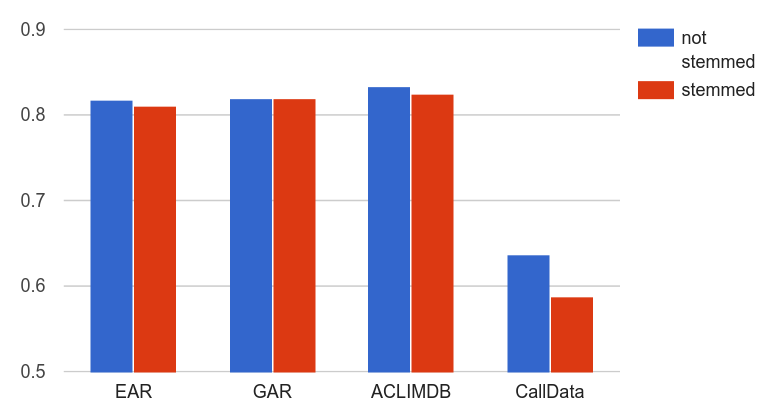
\includegraphics[scale=0.28]{acc-test-bayes}
		\caption{accuracy of Bayes classifier.}
		\label{acc-test-bayes}
	\end{figure}
	
	\paragraph
	One important observation in this experiment is the fact that Naive-Bayes has competitive and sometimes even better results than ANN based methods. But for the call data dataset where there seems to be not enough samples for training a Bayes classifier and the number of shared words in negative and positive training samples are considerably high, it can not compete with the other methods. Specially we have to consider the fact that Bayes method can not utilize the potential of unlabeled data. It would also have the problem of giving a probability to the new words that have never occurred in the training dataset. Also we have to consider that the input of this method for our system would come from an automated speech-to-text system which mean the possibility of having words that are completely out of language vocabulary is very very low. We can also argue the number of words that are used in conversations are much more limited than words used in a written context. We are also assuming that there should be words in conversations of one class that would never occur in the other concept for example in the context of selling products and posting it, words for describing the address would be very less likely to happen in the 'NOT\_SALE' labeled item. This means that we should not completely take the Bayes algorithm off the choices and we should do another experiment with Bayes when more data is available.
	
	\subsection*{ANN based methods}
	ANN(Artificial Neural Networks) and it's variant RNN(Recurrent Neural Networks) based methods specially LSTM have recently shown very good result in almost all the AI problems related to a sequence labeling \cite{Graves2012} \cite{UnreasonableRNN}. To be able to apply them, we have used the adapted code from tflearn library\cite{tflearn2016}(a deep-learning library built on top of Tensorflow\cite{tensorflow2015-whitepaper}) which is using a word embedding layer to transfer text documents into a vector representation. These vectors of words are next fed to an ANN network which at the end was connected to a soft-max layer where the positivity or negativity is decided. There are many hyper parameters that can affect the results of the classifier. Parameters like Optimizer function, Number of epochs(an epoch is a complete training pass through a given dataset), dropout (drop out is a regularization technique where some of the node outputs are randomly set to zero to prevent over-fitting). To find the best hyper parameters and best network architecture we have used several varieties of possible ANN networks. An LSTM(Long Sort Term Memory) network which is a recurrent neural network, A dynamic LSTM network which is an LSTM where the length of input vectors can differ, and a BDRNN(bidirectional recurrent neural network) where it uses the future input in a sequence as well as past input for prediction.\\ 
	To find the best hyper parameters for Optimizer function, we have run the LSTM, BDLST, DLSTM on all the datasets and the results were not dependent on the dataset or the ANN architecture used. Figure \ref{fig:choosingOpitmizer} shows representative result of the mentioned experiment where it illustrates other not only optimizers are not competitive with adam they are on the base line of randomness. maybe prolonging the learning duration eventually lead to convergence of the mentioned methods but this would consume a lot of time and memory resource which is not suggestible.\\

	\begin{figure}
		\centering
		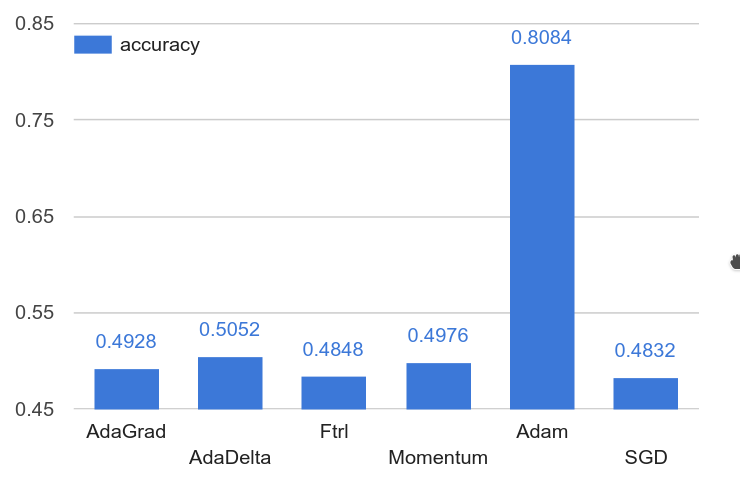
\includegraphics[scale=0.30]{choosingOpitmizer}
		\caption{LSTM accuracy on IMDB reviews dataset using different optimizers}
		\label{fig:choosingOpitmizer}
	\end{figure}
	To find the best number of epochs for the experiments we have compared the best curves on the datasets and realized that 12 epochs can be a reasonable number. Results in the  figure \ref{fig:selectingEpochs} shows classier converges much earlier on aclIMDB dataset which gives us a hint about later comparison between the results of classification on datasets. One possible reason for faster convergence here can be the fact that aclIMDB reviews are all reviews about the same category, while the other datasets are reviews about three different categories.
		\begin{figure}
			\centering
			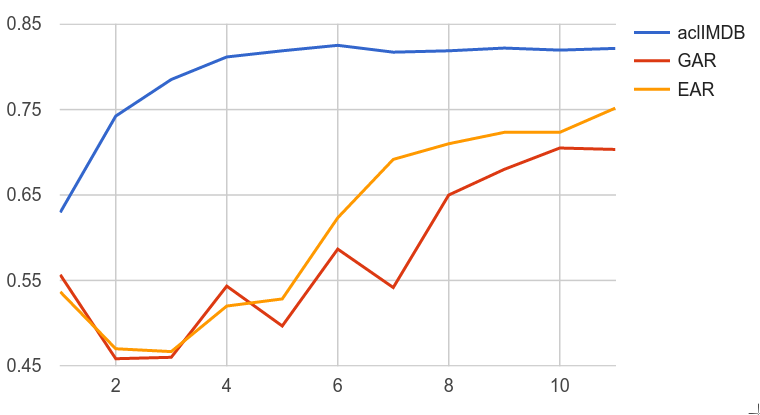
\includegraphics[scale=0.50]{selectingEpochs}
			\caption{Best Leaning curves for each dataset and the number of epochs used }
			\label{fig:selectingEpochs}
		\end{figure}\\
	The experiment for finding the best dropout was the one with the most unexpected results. Our assumption was the dropout should have an almost static nature were above a certain number causes data loss and reduced accuracy and bellow a certain number would cause over-fitting and thus reduced accuracy. To our surprise optimal dropout number is highly Dependant on the nature of data-set.figure \ref{fig:dropoutOnAccuracy} .
	One very interesting observation here was that for GAR(German amazon reviews) dataset, the best drop out was 80\% which is a considerably high number. Another observation is accuracy on German dataset never reaches the accuracy on it's English counterpart which could be due to the German grammar or inflections in German language.
		\begin{figure}
			\centering
			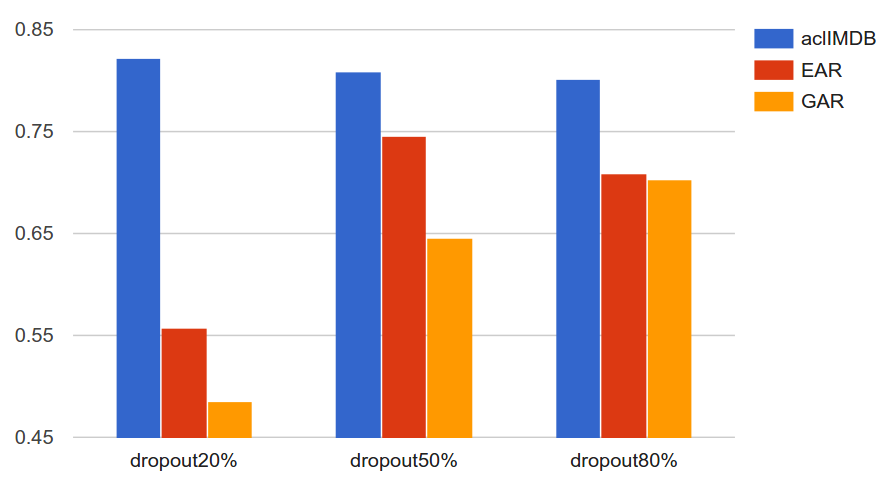
\includegraphics[scale=0.28]{dropoutOnAccuracy}
			\caption{effect of dropout in accuracy on different dataset}
			\label{fig:dropoutOnAccuracy}
		\end{figure}
	\subsection*{vectorized representations of Word and document} 
	The third approach taken in this paper is based on top of embedding algorithms that are utilizing the probability of word distribution regarding their neighbors. These method are transferring words to a high dimensional space where many syntactic and semantic features are captured in the form of distance\cite{explainW2V}. Figure \ref{fig:word2vec-gender-relation}.
	\begin{figure}
		\centering
		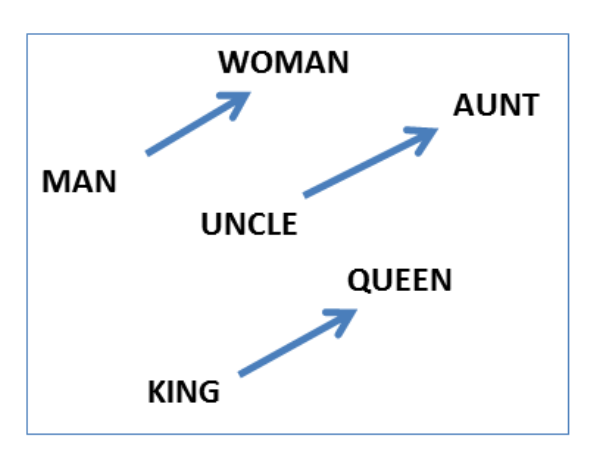
\includegraphics[scale=0.70]{word2vec-gender-relation}
		\caption{Captured semantic information in the form of distance using word2vec algorithm}
		\label{fig:word2vec-gender-relation}
	\end{figure}
	
	\paragraph*
	This representation of words can be used to classify each word as a semantically positive or negative and can also help in sentiment classification of a document. Word2ٰVec\cite{efficentw2v} is one of the most known samples of this method released by google. This method can be run on text corpus in an  unsupervised manner, and it would capture the semantic and syntactic relation between words. This would help the semantic classifier to use this features and apply them also for the words that never happened in the training dataset. This method can be used reliably for finding the semantic polarity of individual words but when the context is bigger then a word for example a sentence, paragraph or a document, it would be important how this individual word vectors are being used to predict a document's polarity. Gensim\cite{gensim} doc2vec which is based on top of word2vec is publicly available code that we have used to combine the individual word vectors into a document vector. This algorithm is first trained on the unsupervised data and later we can get an output vector for a given input document. The output vectors of documents is later fed to a logistic regression layer and a softmax layer to decide the polarity. The network is trained with the train data for 150 epochs where the accuracy converges to a reasonable number with a small tolerance. Table \ref{tbl:doc2vec-accuracy-datasets} shows the final results of using this method which shows very competitive results.
	\begin{table}
		\centering
		\begin{tabular}{| l | l |}
			\hline
			dataset& accuracy \\ \hline
			aclIMDB & 0.8719 \\ \hline
			EAR & 0.7677 \\ \hline
			GAR & 0.7682 \\ \hline
			calldata & 0.84 \\ \hline
		\end{tabular}
		\caption{doc2vec accuracy over different datasets}
		\label{tbl:doc2vec-accuracy-datasets}
	\end{table}\\
	\paragraph*
	the main advantages of this method is the possibility to do unsupervised learning for learning the word vectors which even can be done on other available data from the same language. The second advantage of this method is its fast classifier train time. Also train time for the embedding layer is time and memory exhaustive. Results shows very good output for the aclIMDB dataset which should be due to its relatively large number of available train data. The good results for call-data dataset is our main concern. It seems there are features in this dataset that doc2vec method can exploit. Finding the reasons behind the good results with doc2vec method and trying to improve it can be a part of future works.\\
	One of the concerns that we had about the doc2vec method was, is it conserves the semantic shape of the document? by semantic shape we mean the relation between different parts of text. To confirm this we have fed the output of doc2vec to a LSTM layer and then to a softmax. We assumed if there is relation between the features extracted by doc2vec the learning curve would have a smooth increasing over time. We also wanted to see how adding an LSTM would affect the classifier's results. figure \ref{fig:LSTMdoc2vec} shows that using an LStM layer makes the predictions worse then the previous experiment. The fluctuating values also shows that there is no sequence shape conservation in doc2vec which closes the possibility to use sequence learning approaches on top of doc2vec.\\
	\begin{figure}
		\centering
		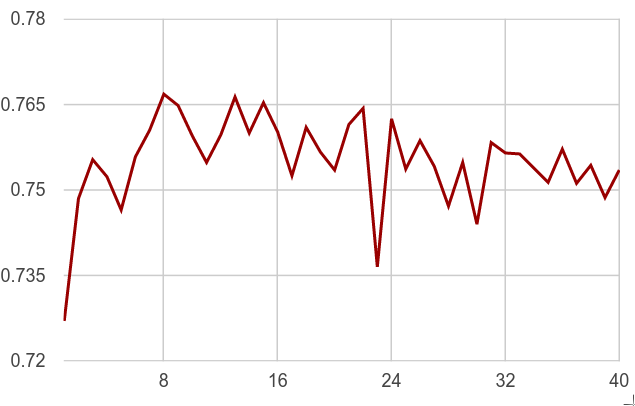
\includegraphics[scale=0.50]{LSTMdoc2vec}
		\caption{Accuracy of LSTM classifier on top doc2vec input}
		\label{fig:LSTMdoc2vec}
	\end{figure}
	\paragraph*
	Fasttext library\cite{enrichWordvecs-with-subwords}\cite{Bag-of-Tricks} which is the latest try of Facebook for getting an efficient representation of word in vector space is also another method which has been used here for comparison. Fast text library comes with an inbuilt text classifier which we have used to compare it with the out put of Doc2vec-logistic classifier. The most important advantage of facebook fasttext is, very time and memory efficient implementation of the algorithm, where training and testing time is remarkably fast. Table \ref{tbl:fasttext-accuracy-datasets } shows the results of using fast-text algorithm for classification
	\begin{table}
		\centering
		\begin{tabular}{| l | l |}
			\hline
			dataset& accuracy \\ \hline
			aclIMDB & 0.85 \\ \hline
			EAR &   0.756 \\ \hline
			GAR &   0.762 \\ \hline
			calldata & 0.83  \\ \hline
		\end{tabular}
		\caption{fast-text algorithm accuracy over different datasets}
		\label{tbl:fasttext-accuracy-datasets  }
	\end{table}

\section{Conclusion}
	Transcribed data from Phone conversations in Matelso GMBH has a few main features. 1-the sample size is limited 2- conversations are transcribed using Bing automated text to speech recognition system and a percentage of tolerance for words being mistakenly transcribed should be considered. 3- the text is result of transcription of a conversation so repetition and not following correct grammar is very likely. By taking into account the special features for call data we realize the methods like LSTM or BDLSTM which are trying to use the sequential structure of data as an important feature are not performing as good as methods which are using semantic polarity of individual words and sentences. We also realize due to shortage of train dataset which would be the case for most similar experiments on voice data Bayes method would not be satisfactory enough. Best recorded result in our experiments was with Doc2vec method, and we would suggest industry or other researchers to use this method for the analysis.
	
\section{Future works}
	There can be many more classes of data that are useful for the purpose of marketing and evaluation which can be used to evaluate these methods in a future work.\\
	The voice data can also have features like tone, etc which maybe possible to be exploited in the classification. working on the voice data and extracting features from it can be a future work. 
\section{Acknowledgements}
	call-data dataset and the resources for using it and the labeling process on this data has been done with the help of MATELSO GMBH

%

%
% ---- Bibliography ----
%
\bibliographystyle{unsrt}
\bibliography{bibexample}
%
\end{document}
